
\section{Principali polimeri coniugati donatori}
\nsub{Basati su $p$-fenilene vinilene}
\footnotesize{Via Wessling, la via storica:}
\begin{figure}{\centering{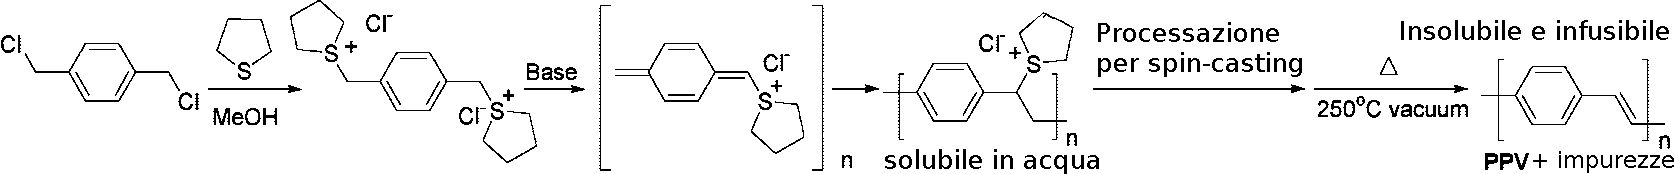
\includegraphics[width=1\textwidth]{img/ppv2.png}}}\end{figure}
\footnotesize{Via Glich (i gruppi alcossi abbassano il LUMO):}
\begin{figure}{\centering{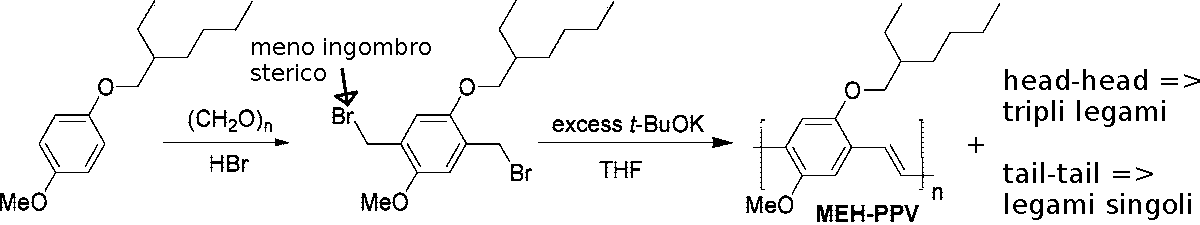
\includegraphics[width=0.85\textwidth]{img/ppv-meh.png}}}\end{figure}
\footnotesize{Via Wittig-Horner per avere maggiore regioregolarità:}
\begin{figure}{\centering{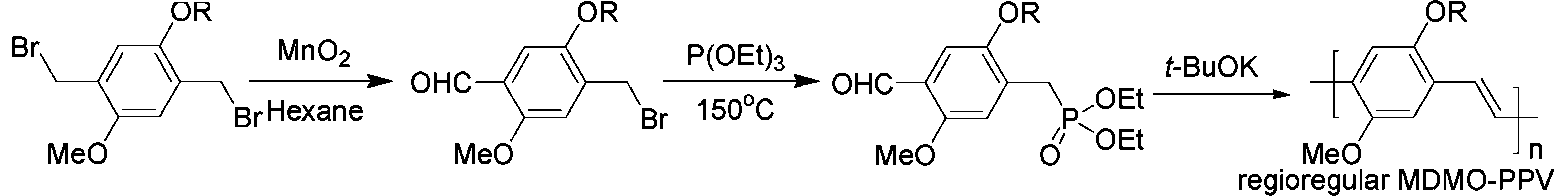
\includegraphics[width=0.95\textwidth]{img/ppv-wittig.png}}}\end{figure}
\end{frame}
%%%%%%%%%%%%%%%%%%%%%%%%%%%%%%%%%%%%%%%%%%%%%%%%%%%%%%%%%%%%%%%%%%%%%%%%%%%%%%%%%%%%%%%%%%%%%%%%%%%%%%%%%%%%%%%%%%%%%%%%%%%%%%
\subsubsection{Variazioni sulla struttura}\begin{frame}\frametitle{Basati su $p$-fenilene vinilene}\framesubtitle{Variazioni sulla struttura}
 \begin{columns}
\column{0.3\linewidth} 
{Aumentato assorbimento e trasporto lacune. Diminuito \emph{band~gap}.}
\begin{figure}{\centering{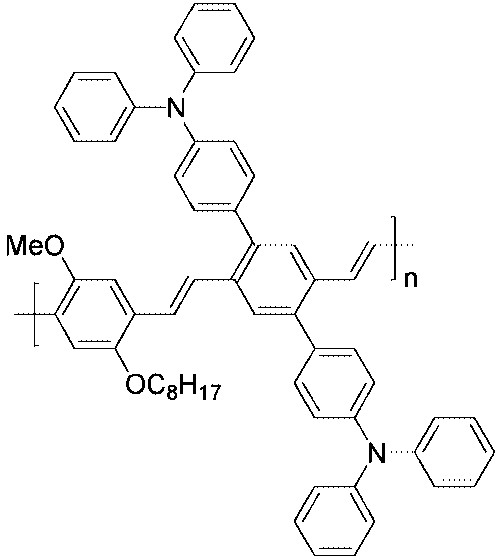
\includegraphics[width=1\textwidth]{img/ppv-ammina.png}}}\end{figure}
\column{0.7\linewidth}
{Tiofene elettronricco e poco aromatico, \emph{band gap} minore. Polimerizzazione ossidativa con \ce{FeCl3}.}
\vspace{-15pt}\begin{figure}{\centering{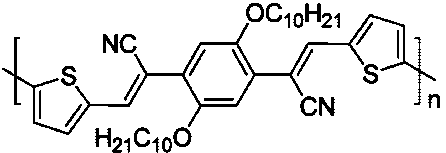
\includegraphics[width=0.5\textwidth]{img/ppv-cn-tio.png}}}\end{figure}
{Più linearità quindi migliore cristallizzazione.}
\begin{figure}{\centering{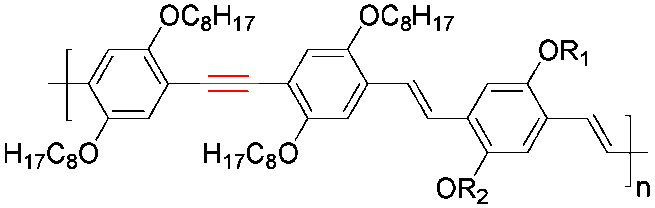
\includegraphics[width=0.8\textwidth]{img/ppv-ino.png}}}\end{figure}

\end{columns}
\end{frame}
\nsub{Basati su fluorene}
Vantaggi dei polimeri a base di 9,9-dialchilfluorene:
\begin{itemize}
 \item ottima conduzione di lacune: $I_{short-circuit}$ maggiori;
 \item possibile ottenere film;
 \item stabilità alle ossidazioni: HOMO basso, $V_{open-circuit}$ maggiori;
\end{itemize}
Svantaggio: \emph{band gap} troppo grande (scarso assorbimento).

Per diminuire il \emph{band gap} si polimerizza un dimero fluorene-composto elettron-ricco (bitiofene o pentacene o antraditiofene) via Suzuki:
\begin{figure}{\centering{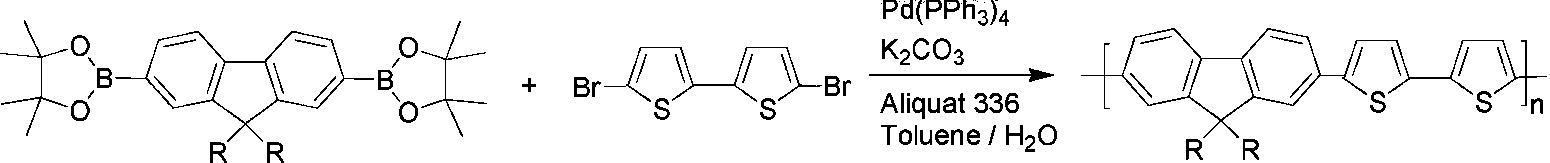
\includegraphics[width=1\textwidth]{img/fluo-tio.png}}}\end{figure}

\end{frame}
\subsubsection{Utilizzo di gruppi ausiliari}\begin{frame}\frametitle{Basati su fluorene}\framesubtitle{Utilizzo di gruppi ausiliari}
\begin{columns}\column{0.6\linewidth}Oppure si può utilizzare un monomero contenente unità elettron-donatori (tiofene) e elettron-accettori (2,1,3-benzotiadiazolo) per ottenere una nuova banda di assorbimento a $\lambda$ grandi per il trasferimento di carica.
\column{0.4\linewidth}\vspace{-35pt}\begin{figure}{\centering{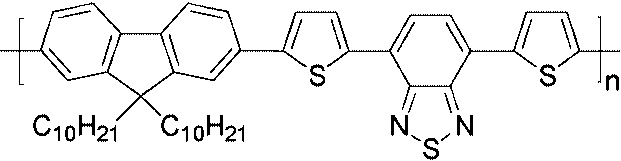
\includegraphics[width=1\textwidth]{img/fluo-tiaza.png}}}\end{figure}
\end{columns}\vspace{10pt}
\begin{columns}\column{0.5\linewidth}\begin{figure}{\centering{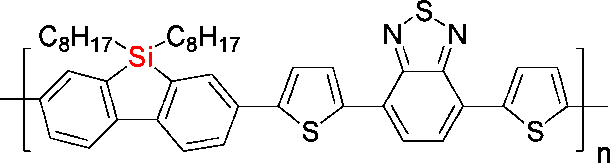
\includegraphics[width=1\textwidth]{img/fluo-si.png}}}\end{figure}
\column{0.6\linewidth}Sostituendo il C9 con Si si ottiene una diminuzione del \emph{band gap} (più assorbimento; silolo ha $\Delta E_{HOMO-LUMO}$ piccolo), un abbassamento del HOMO ($V_{open-circuit}$ maggiore) e altissima mobilità di lacune.
\end{columns}

\end{frame}

%%%%%%%%%%%%%%%%%%%%%%%%%%%%%%%%%%%%%%%%%%%%%%%%%%%%%%%%%%%%%%%%%%%%%%%%%%%%%%%%%%%%%%%%%%%%%%%%%%%%%%%%%%%%%%%%%%%%%%%%%%%%%%
\logo{}
\nsub{Basati su carbazolo}
L'azoto 
rende aromatico e elettron-donatore il carbazolo. Forma cationi stabili ed ha una buona mobilità di lacune.

\vspace{-6pt}\begin{figure}{\centering{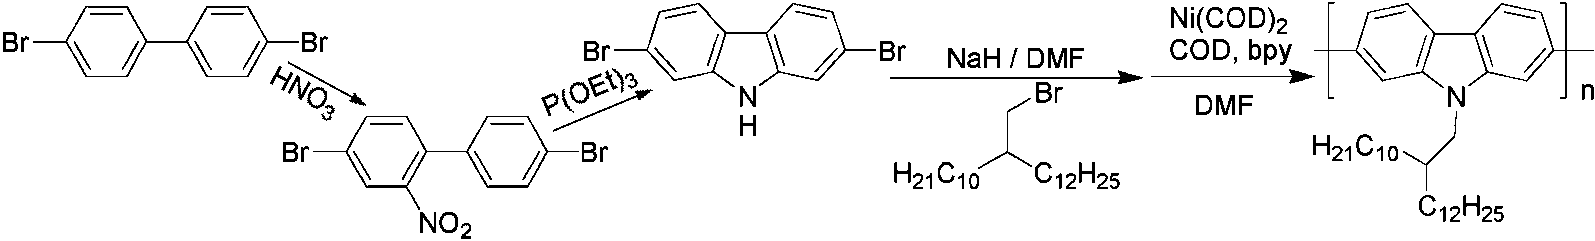
\includegraphics[width=1\textwidth]{img/carbaz-sint.png}}}\end{figure}
\vspace{-12pt}Unità elettron-attrattrici incorporate per abbassare il \emph{band gap}.\\ Sistemi indolocarbazolo più donatori e più cristallini (più conduzione e più assorbimento).
\vspace{-10pt}\begin{columns}\column{0.4\linewidth}\begin{figure}{\centering{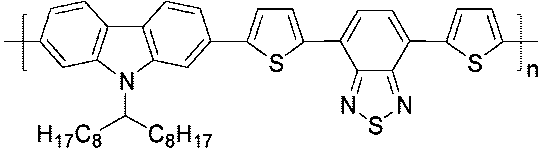
\includegraphics[width=1\textwidth]{img/carbaz-tio.png}}}\end{figure}\column{0.6\linewidth}\begin{figure}{\centering{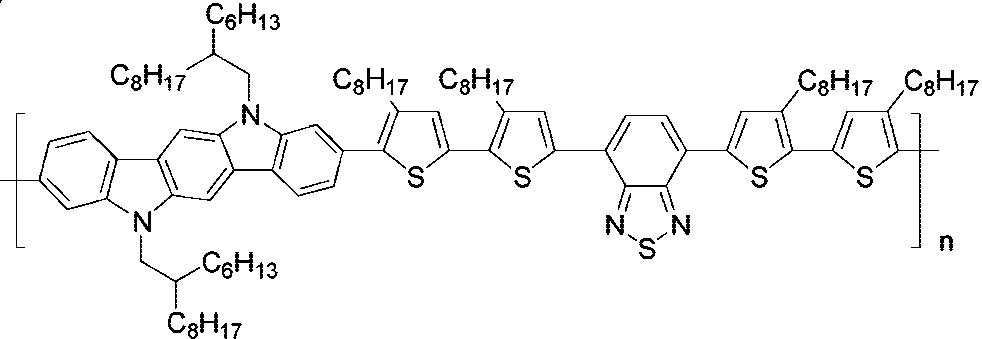
\includegraphics[width=1\textwidth]{img/carbaz-indolo.png}}}\end{figure}\end{columns}
\end{frame}
\logo{
\includegraphics[width=0.07\paperwidth]{img/snslogo.png}}

%%%%%%%%%%%%%%%%%%%%%%%%%%%%%%%%%%%%%%%%%%%%%%%%%%%%%%%%%%%%%%%%%%%%%%%%%%%%%%%%%%%%%%%%%%%%%%%%%%%%%%%%%%%%%%%%%%%%%%%%%%%%%%
\nsub{Basati su tiofene}
Molto impiegato è il poli(3-esiltiofene) regioregolare \emph{head-tail}, 
\begin{itemize}
 \item una catena laterale più corta non rende solubile il polimero, più lunga favorisce la separazione di fase nella cella solare;
 \item regioregolarità per avere planarità (coniugazione) e cristallinità (conduzione intercatena e assorbimento);
 \item cristallinità se eccessiva provoca separazione di fase durante la fase di \emph{annealing} (perciò si inseriscono difetti nella catena tramite un comonomero); se troppo scarsa (per catene troppo corte) si ha difficile conduzione intercatena e minore assorbimento.
\end{itemize}\end{frame}
\subsubsection{Ciclo catalitico della polimerizzazione}\begin{frame}\frametitle{Basati su tiofene}\framesubtitle{Ciclo catalitico della polimerizzazione}
\small{La sintesi via metatesi Grignard e coupling di Kumada-Corriu porta a una polimerizzazione vivente con bassa polidispersità. }
\begin{figure}{\centering{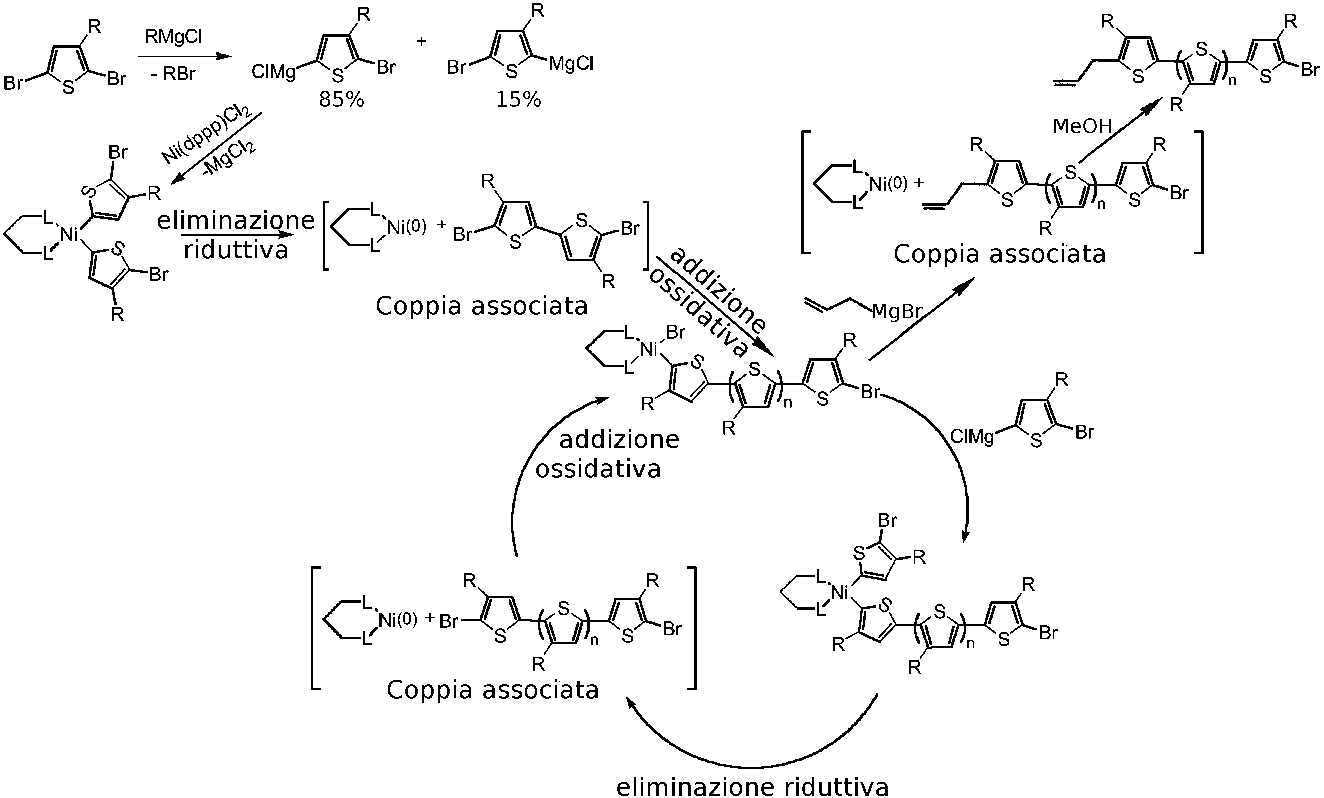
\includegraphics[width=0.85\textwidth]{img/pol-grim-polimerizz3.png}}}\end{figure}
\end{frame}





\subsubsection{Politiofene con catene laterali coniugate}\begin{frame}\frametitle{Basati su tiofene}\framesubtitle{Politiofene con catene laterali coniugate}
Gruppi laterali coniugati per aumentare l'assorbimento.
\begin{columns}\column{0.6\linewidth}Inoltre HOMO abbassato: $V_{open-circuit}$ maggiore senza perdita di assorbimento.
\column{0.4\linewidth}\vspace{-20pt}\begin{figure}{\centering{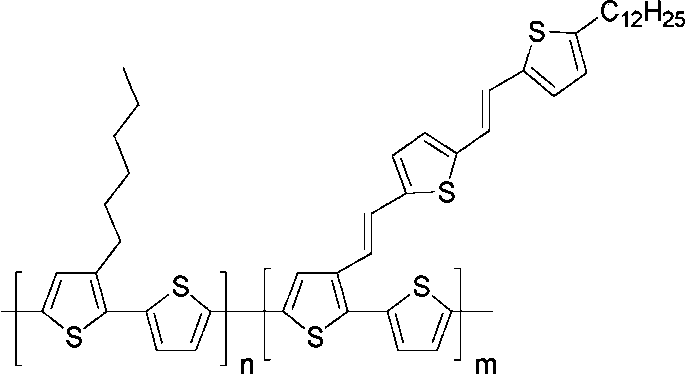
\includegraphics[width=1\textwidth]{img/p3ht-conj-tio.png}}}\end{figure}
\end{columns}\vspace{-20pt}
\begin{columns}\column{0.3\linewidth}\begin{figure}{\centering{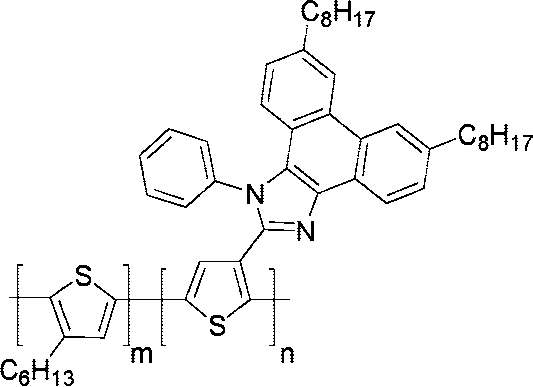
\includegraphics[width=1\textwidth]{img/p3ht-conj-accept.png}}}\end{figure}
\column{0.7\linewidth}Inoltre accettore intermedio di $e^-$: facilita il trasferimento al materiale accetore.
\end{columns}\vspace{5pt}
Dei politiofeni reticolati con ponti coniugati per aumentare la mobilità di lacune hanno mostrato peggioramento delle caratteristiche a causa della deformazione indotta.
\end{frame}




\subsubsection{Politiofene con anelli fusi in 3,4}\begin{frame}\frametitle{Basati su tiofene}\framesubtitle{Politiofene con anelli fusi in 3,4}
\begin{columns}
\column{0.25\linewidth}
\begin{figure}{\centering{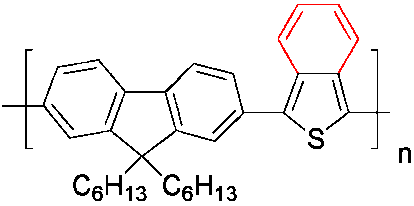
\includegraphics[width=1.1\textwidth]{img/tio-fus-benz-fluo.png}}}\end{figure}
\column{0.75\linewidth}Fondendo un anello benzenico sull'anello tiofenico si aumenta il peso della forma chinonica e si ottengono (per polimerizzazione elettrochimica, termica o ossidativa con \ce{FeCl3}) polimeri con \emph{band gap} e peso molecolare troppo bassi e con scarsa stabilità chimica. Può essere utilizzato in con fluorene per abbassarne il \emph{band gap}.
\end{columns}
\vspace{10pt}\begin{columns}
\column{0.6\linewidth}Anche il tieno[3,4-$b$]tiofene può servire per abbassare il \emph{band gap} a seconda del contenuto nel polimero. Nella figura la catena perfluorurata stabilizza l'anello elettronricco.
\column{0.3\linewidth}\vspace{-20pt}\begin{figure}{\centering{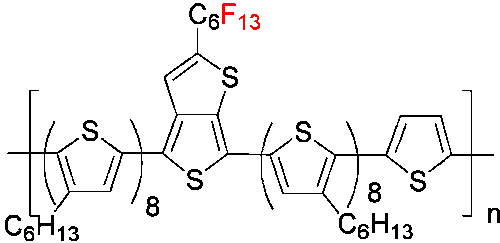
\includegraphics[width=1\textwidth]{img/tio-fus-tio.png}}}\end{figure}
\end{columns}
\end{frame}


\subsubsection{Politiofene con anelli fusi in 2,3}\begin{frame}\frametitle{Basati su tiofene}\framesubtitle{Politiofene con anelli fusi in 2,3}
Un carbonio a ponte aumenta la planarità e diminuisce il \emph{band gap}.\vspace{10pt}\begin{columns}\column{0.5\linewidth}
Il gruppo elettron-attrattore diminuisce il \emph{band gap} ed aumenta le interazioni intermolecolari. Il secondo blocco assorbe a frequenze diverse. 
\column{0.5\linewidth}
\begin{figure}{\centering{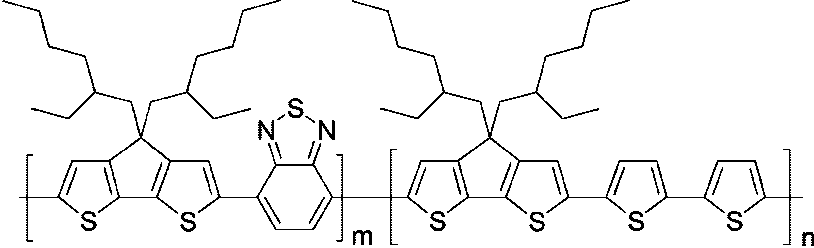
\includegraphics[width=1\textwidth]{img/tio-fus-penta.png}}}\end{figure}
\end{columns}
\begin{columns}\column{0.3\linewidth}\begin{figure}{\centering{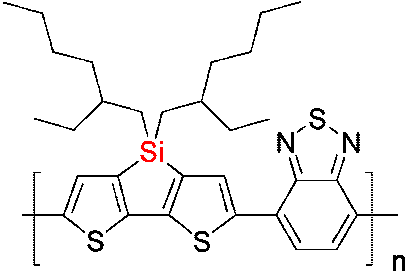
\includegraphics[width=1\textwidth]{img/tio-fus-si.png}}}\end{figure}
\column{0.6\linewidth}Come nel fluorene, usare un Si come ponte permette di avere mobilità elettroniche 3 volte maggiori, HOMO più basso e assorbimento fino a 800nm (\emph{band gap} minore).
\end{columns}
\end{frame}



\subsubsection{Politiofene con vinileni o etinileni}\begin{frame}\frametitle{Basati su tiofene}\framesubtitle{Politiofene con vinileni o etinileni}
\begin{columns}
\column{0.3\linewidth}
\vspace{-10pt}
\begin{figure}{\centering{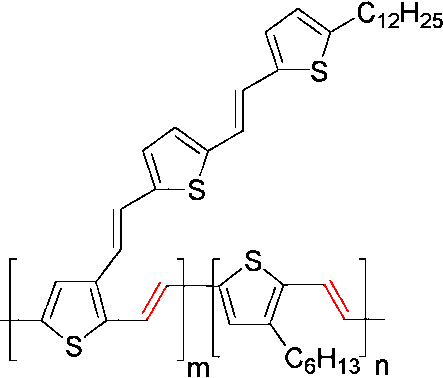
\includegraphics[width=1\textwidth]{img/tio-vinilene.png}}}\end{figure}
\column{0.7\linewidth}
Inserendo unità vinilene si riduce l'aromaticità, aumenta la planarità, la coniugazione, si assorbe molto più spettro. Per aggirare problemi di difficile processabilità è possibile rendere coniugato il polimero \emph{in situ}. 
\end{columns}
\begin{columns}
\column{0.6\linewidth}Il triplo legame da rigidità ed aumenta la coniugazione. Nella figura un gruppo donatore ed uno accettore danno un polimero con basso \emph{band gap}.
\column{0.3\linewidth}\begin{figure}{\centering{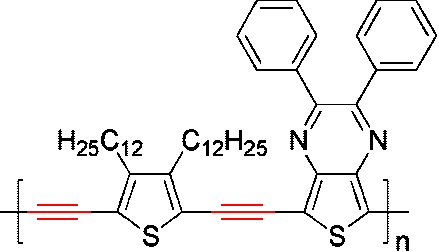
\includegraphics[width=1\textwidth]{img/tio-ino.png}}}\end{figure}
\end{columns}
\end{frame}





%%%%%%%%%%%%%%%%%%%%%%%%%%%%%%%%%%%%%%%%%%%%%%%%%%%%%%%%%%%%%%%%%%%%%%%%%%%%%%%%%%%%%%%%%%%%%%%%%%%%%%%%%%%%%%%%%%%%%%%%%%%%%%

\nsub{Esempi di altri polimeri donatori}
\begin{columns}
\column{0.6\linewidth}Una politriarilammina non è coniugata lungo la catena a causa dell'azoto e non è planare. Ciò nonostante, grazie alla coppia con un gruppo elettron-attrattore, può avere un basso \emph{band gap}.
\column{0.4\linewidth}
\begin{figure}{\centering{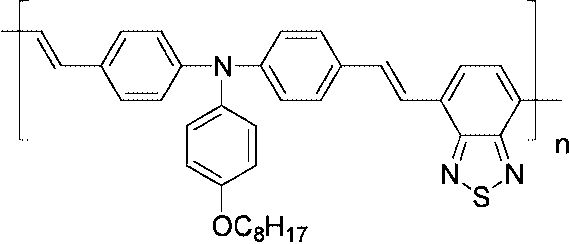
\includegraphics[width=1\textwidth]{img/ammina.png}}}\end{figure}
\end{columns}
\vspace{10pt}
\begin{columns}
\column{0.5\linewidth}\vspace{-10pt}\begin{figure}{\centering{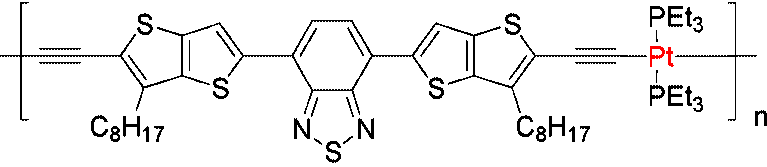
\includegraphics[width=1\textwidth]{img/platino.png}}}\end{figure}
\column{0.5\linewidth}Un atomo di platino permette un efficiente \emph{intersystem crossing} formando stati eccitati di tripletto ossia eccitoni con tempi di vita più lunghi e minore ricombinazione di cariche.
\end{columns}
\end{frame}

